\section{\textcolor[HTML]{D32F2F}{Oppgaven}}

\subsection{Problembeskrivelse}
Gruppen fikk i oppgave å kartlegge behovet for en app på Sirkus Shopping, et kjøpesenter i Trondheim. Gruppen skulle gå gjennom hele prosessen, fra observasjoner og intervjuer, til prototyping, testing og utvikling av et ferdig produkt. Fokuset skulle ligge på brukersentrert design og iterative prosesser. 
\\\\
Sirkus shopping er et kjøpesenter på Persaunet i Trondheim. Her er det rundt 100 butikker, samt mange parkeringsplasser og lett tilgjengelighet med kollektivtransport. Målgruppen for kjøpesenteret er småbarnsforeldre og studenter, noe som gjenspeiles i butikkene på senteret.  Her finner man alt fra bokhandel, babybutikker og gullsmed til leketøysbutikk og hudklinikk\cite{sirkus}. Logoen til kjøpesenteret er vist i Figur \ref{fig:sirkus}.

\begin{figure}[H]
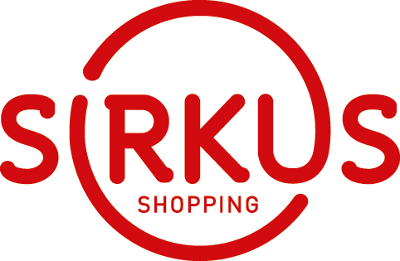
\includegraphics[scale=0.6]{images/sirkus}
\centering %centering the image
\caption{Logo Sirkus shopping}
\label{fig:sirkus}
\end{figure}

\subsection{Kravspesifikasjon}
Prosjektoppgaven gruppen fikk presentert omhandlet å forbedre shoppingopplevelsen. Oppgaven gikk ut på å bruke den nye generasjonen mobiltelefoner på nye måter. Her var \textit{iPhone} og \textit{Android} trukket fram som eksempler, hvor man skulle finne en måte å bruke teknologien i sammenheng med alt man gjør på et handlesenter. Målgruppen var kunder på et kjøpesenter, hvor hver gruppe fikk tildelt et spesifikt senter. Her skulle gruppen observere og intervjue målgruppen, og gjennom dette finne ut hva de kunne ønske seg i en app. Dette skulle gruppen så lage en prototype av, og teste på faktiske brukere.
\\\\
Det ble gitt flere retningslinjer for løsningen gruppen skulle lage. De fire viktigste kravene var brukbarhet, selvmotivasjon, innhold og dialog. I brukbarhet ligger det at produktet skal være selvforklarende og intuitivt å bruke. I selvmotivasjon ligger det at produktet skal være laget slik at desto mer tid brukeren bruker sammen med produktet, eller i appen, desto mer lyst skal brukeren ha til å bruke produktet. Innholdet i produktet skulle gi korrekt informasjon, slik at kunden kunne stole på det produktet ga av opplysninger. Til slutt var det krav om dialog. I det ligger det at produktet skulle være et resultat av dialog med potensielle brukere, i form av feltstudier, intervjuer og brukertester.
\\\\
I oppgaveteksten ble det spesifisert at produktet skulle være laget for iPhone og/eller Android, uten at dette krevde at gruppene behøvde å lage prototypene eksakt likt disse designene. iPhone og Android er begge smarttelefoner med en rekke sensorer, samt kontinuerlig tilkobling til Internett. Dette gir mange muligheter, hvor man kan ta i bruk sosiale medier eller Internet of Things. Smarte klokker er også nevnt som en mulighet, hvor klokken snakker med smarttelefonen via Bluetooth og kan styre appen herfra. I tillegg til dette, ble også QR-koder og beacons presentert som teknologier, \ref{teknologiundersokelse}.
\\\\
\noindent Prosjektet var tydelig delt opp i følgende segmenter:
\begin{itemize}
    \item\textbf{Forståelse av oppgave:} (Kan leses om i Kapittel \ref{tjenestedesign})
    \begin{itemize}
        \item Observasjon og analyse av tildelt senter med personer og handlemønster.
        \item Samling av data i form av intervju og spørreundersøkelse.
        \item Definere målgruppe, personas og scenarier basert data.
    \end{itemize}
    \item\textbf{Konseptutvikling:} (Kan leses om i Kapittel \ref{konseptet})
    \begin{itemize}
        \item Konseptutvikling på grunnlag av aktiviteter i 1.
    \end{itemize}
    \item\textbf{Design iterasjon 1:} (Kan leses om i Kapittel \ref{design1})
    \begin{itemize}
        \item Papirprototyping med brukertester.
    \end{itemize}
    \item\textbf{Design iterasjon 2:} (Kan leses om i Kapittel \ref{design2})
    \begin{itemize}
        \item Redesign med Axure og eyetracking.
    \end{itemize}
    \item\textbf{Evaluering, refleksjon og videre utvikling}. (Kan leses om i Kapittel \ref{videre} og Kapittel \ref{oppsummering})
\end{itemize}





% Gruppen tolket oppgaven som at studentene skulle reise til Sirkus shopping og observere kundene og deres adferd. I neste runde skulle studentene intervjue kunder og samle data. Med resultatene fra undersøkelsene skulle gruppen lage et sett med personas som kunne representere en eller flere typiske kunder på kjøpesenteret, samt lage scenario for når produktet kunne brukes.
% Ved å analysere resultater og studere personas skulle gruppen komme opp med en idé på noe som kunne løse en utfordring kunden hadde, eller noe som kunne gjøre handleopplevelsen bedre. Deretter skulle gruppen lage en papirprototype av løsningen, som skulle testes på brukere. Resultatene fra brukertesten skulle gruppen ta med videre i utviklingen av neste prototyp, som skulle lages i et program kalt Axure. Her skulle gruppen teste flere funksjonaliteter, og testingen skulle foregå med eyetracking på lab. Resultatene fra denne brukertesten skulle brukes til å videreutvikle et tredje design for produktet.\\\\